%%%%%%%%%%%%%%%%%%%%%%%%%%%%%%%%%%%%%%%%%%%%%%%%%%%%%%%
% Please note that whilst this template provides a
% preview of the typeset manuscript for submission, it
% will not necessarily be the final publication layout.
%
% letterpaper/a4paper: US/UK paper size toggle
% num-refs/alpha-refs: numeric/author-year citation and bibliography toggle

%\documentclass[letterpaper]{oup-contemporary}
\documentclass[a4paper,num-refs]{oup-contemporary}

%%% Journal toggle; only specific options recognised.
%%% (Only "gigascience" and "general" are implemented now. Support for other journals is planned.)
\journal{gigascience}

\usepackage{graphicx}
\usepackage{siunitx}

% Additional packages for data model figure
\usepackage{forest}
\usepackage{tikz}
\usetikzlibrary{quotes,arrows.meta,3d}

% Local definitions to systematise tool naming
\newcommand{\sgapi}[1]{\texttt{#1}}
\newcommand{\toolname}[1]{\texttt{#1}}
\newcommand{\sgkit}{\texttt{sgkit}}


%%% Flushend: You can add this package to automatically balance the final page, but if things go awry (e.g. section contents appearing out-of-order or entire blocks or paragraphs are coloured), remove it!
% \usepackage{flushend}

% Macros etc for data model figure
% TODO: simplify this code
% flexible cuboid from
% https://tex.stackexchange.com/questions/267982/tikz-easy-drawing-of-cuboids
\makeatletter
\def\tikz@lib@cuboid@get#1{\pgfkeysvalueof{/tikz/cuboid/#1}}
\def\tikz@lib@cuboid@setup{%
	\pgfmathsetlengthmacro{\vxx}%
	{\tikz@lib@cuboid@get{xscale}*cos(\tikz@lib@cuboid@get{xangle})*1cm}
	\pgfmathsetlengthmacro{\vxy}%
	{\tikz@lib@cuboid@get{xscale}*sin(\tikz@lib@cuboid@get{xangle})*1cm}
	\pgfmathsetlengthmacro{\vyx}%
	{\tikz@lib@cuboid@get{yscale}*cos(\tikz@lib@cuboid@get{yangle})*1cm}
	\pgfmathsetlengthmacro{\vyy}%
	{\tikz@lib@cuboid@get{yscale}*sin(\tikz@lib@cuboid@get{yangle})*1cm}
	\pgfmathsetlengthmacro{\vzx}%
	{\tikz@lib@cuboid@get{zscale}*cos(\tikz@lib@cuboid@get{zangle})*1cm}
	\pgfmathsetlengthmacro{\vzy}%
	{\tikz@lib@cuboid@get{zscale}*sin(\tikz@lib@cuboid@get{zangle})*1cm}
}

\def\tikz@lib@cuboid@draw#1--#2--#3\pgf@stop{%
	\begin{scope}[join=bevel,x={(\vxx,\vxy)},y={(\vyx,\vyy)},z={(\vzx,\vzy)}]
		% first fill the faces with global and individual style
		% then draw the grids
		\begin{scope}[canvas is yz plane at x=#1]
			\draw[cuboid/all faces,cuboid/edges,cuboid/right face] 
			(0,0) -- ++(#2,0) -- ++(0,-#3) -- ++(-#2,0) -- cycle;
			\draw[cuboid/all grids,cuboid/right grid] (0,0) grid (#2,-#3);
		\end{scope}
		\begin{scope}[canvas is xy plane at z=0]
			\draw[cuboid/all faces,cuboid/edges,cuboid/front face] 
			(0,0) -- ++(#1,0) --  ++(0,#2) -- ++(-#1,0) -- cycle;
			\draw[cuboid/all grids,cuboid/front grid] (0,0) grid (#1,#2);
		\end{scope}
		\begin{scope}[canvas is xz plane at y=#2]
			\draw[cuboid/all faces,cuboid/edges,cuboid/top face] 
			(0,0) -- ++(#1,0) --  ++(0,-#3) -- ++(-#1,0) -- cycle;
			\draw[cuboid/all grids,cuboid/top grid] (0,0) grid (#1,-#3);
		\end{scope}
		% now, draw the hidden edges
		\draw[cuboid/hidden edges] (0,#2,-#3) -- (0,0,-#3) -- (0,0,0) 
		(0,0,-#3) -- ++(#1,0,0);
		% finally, draw the visible edges 
		\begin{scope}[canvas is yz plane at x=#1]
			\draw[cuboid/all faces,cuboid/right face,cuboid/edges,fill opacity=0] 
			(0,0) -- ++(#2,0) -- ++(0,-#3) -- ++(-#2,0) -- cycle;
		\end{scope}
		\begin{scope}[canvas is xy plane at z=0]
			\draw[cuboid/all faces,cuboid/front face,cuboid/edges,fill opacity=0] 
			(0,0) -- ++(#1,0) --  ++(0,#2) -- ++(-#1,0) -- cycle;
		\end{scope}
		\begin{scope}[canvas is xz plane at y=#2]
			\draw[cuboid/all faces,cuboid/top face,cuboid/edges,fill opacity=0] 
			(0,0) -- ++(#1,0) --  ++(0,-#3) -- ++(-#1,0) -- cycle;
		\end{scope}
		% define the anchors: 8 vertices
		\path (0,#2,0) coordinate (-left top front)
		coordinate (-left front top)
		coordinate (-top left front)
		coordinate (-top front left)
		coordinate (-front top left)
		coordinate (-front left top);
		\path (0,#2,-#3) coordinate (-left top rear)
		coordinate (-left rear top)
		coordinate (-top left rear)
		coordinate (-top rear left)
		coordinate (-rear top left)
		coordinate (-rear left top);
		\path (0,0,-#3) coordinate (-left bottom rear)
		coordinate (-left rear bottom)
		coordinate (-bottom left rear)
		coordinate (-bottom rear left)
		coordinate (-rear bottom left)
		coordinate (-rear left bottom);
		\path (0,0,0) coordinate (-left bottom front)
		coordinate (-left front bottom)
		coordinate (-bottom left front)
		coordinate (-bottom front left)
		coordinate (-front bottom left)
		coordinate (-front left bottom);
		\path (#1,#2,0) coordinate (-right top front)
		coordinate (-right front top)
		coordinate (-top right front)
		coordinate (-top front right)
		coordinate (-front top right)
		coordinate (-front right top);
		\path (#1,#2,-#3) coordinate (-right top rear)
		coordinate (-right rear top)
		coordinate (-top right rear)
		coordinate (-top rear right)
		coordinate (-rear top right)
		coordinate (-rear right top);
		\path (#1,0,-#3) coordinate (-right bottom rear)
		coordinate (-right rear bottom)
		coordinate (-bottom right rear)
		coordinate (-bottom rear right)
		coordinate (-rear bottom right)
		coordinate (-rear right bottom);
		\path (#1,0,0) coordinate (-right bottom front)
		coordinate (-right front bottom)
		coordinate (-bottom right front)
		coordinate (-bottom front right)
		coordinate (-front bottom right)
		coordinate (-front right bottom);
		% centers of the 6 faces
		\coordinate (-left center) at (0,.5*#2,-.5*#3);
		\coordinate (-right center) at (#1,.5*#2,-.5*#3);
		\coordinate (-top center) at (.5*#1,#2,-.5*#3);
		\coordinate (-bottom center) at (.5*#1,0,-.5*#3);
		\coordinate (-front center) at (.5*#1,.5*#2,0);
		\coordinate (-rear center) at (.5*#1,.5*#2,-#3);
		% center of the cuboid
		\coordinate (-center) at (.5*#1,.5*#2,-.5*#3);
		% centers of the 12 edges
		\path (0,#2,-.5*#3) coordinate (-left top center) 
		coordinate (-top left center);
		\path (.5*#1,#2,-#3) coordinate (-top rear center)
		coordinate (-rear top center);
		\path (#1,#2,-.5*#3) coordinate (-right top center)
		coordinate (-top right center);
		\path (.5*#1,#2,0) coordinate (-top front center)
		coordinate (-front top center);
		\path (0,0,-.5*#3) coordinate (-left bottom center) 
		coordinate (-bottom left center);
		\path (.5*#1,0,-#3) coordinate (-bottom rear center)
		coordinate (-rear bottom center);
		\path (#1,0,-.5*#3) coordinate (-right bottom center)
		coordinate (-bottom right center);
		\path (.5*#1,0,0) coordinate (-bottom front center)
		coordinate (-front bottom center);
		\path (0,.5*#2,0) coordinate (-left front center) 
		coordinate (-front left center);
		\path (0,.5*#2,-#3) coordinate (-left rear center)
		coordinate (-rear left center);
		\path (#1,.5*#2,0) coordinate (-right front center)
		coordinate (-front right center);
		\path (#1,.5*#2,-#3) coordinate (-right rear center)
		coordinate (-rear right center);
	\end{scope}
}

\tikzset{
	pics/cuboid/.style = {
		setup code = \tikz@lib@cuboid@setup,
		background code = \tikz@lib@cuboid@draw#1\pgf@stop
	},
	pics/cuboid/.default={1--1--1},
	cuboid/.is family,
	cuboid,
	all faces/.style={fill=white},
	all grids/.style={draw=none},
	front face/.style={},
	front grid/.style={},
	right face/.style={},
	right grid/.style={},
	top face/.style={},
	top grid/.style={},
	edges/.style={},
	hidden edges/.style={draw=none},
	xangle/.initial=0,
	yangle/.initial=90,
	zangle/.initial=210,
	xscale/.initial=1,
	yscale/.initial=1,
	zscale/.initial=0.5
}

\newcommand{\tikzcuboidreset}{
	\tikzset{cuboid,
		all faces/.style={fill=white},
		all grids/.style={draw=none},
		front face/.style={},
		front grid/.style={},
		right face/.style={},
		right grid/.style={},
		top face/.style={},
		top grid/.style={},
		edges/.style={},
		hidden edges/.style={draw=none},
		xangle=0,
		yangle=90,
		zangle=225,
		xscale=1,
		yscale=1,
		zscale=0.5
	}
}

\newcommand{\tikzcuboidset}{\@ifstar\tikzcuboidset@star\tikzcuboidset@nostar} 
\newcommand{\tikzcuboidset@nostar}[1]{\tikzcuboidreset\tikzset{cuboid,#1}}
\newcommand{\tikzcuboidset@star}[1]{\tikzset{cuboid,#1}}
\makeatother


% See https://github.com/sgkit-dev/vcf-zarr-publication/issues/87
% for discussion
\title{Analysis-ready VCF at Biobank scale using Zarr}

%%% Use the \authfn to add symbols for additional footnotes, if any. 
% 1 is reserved for correspondence emails; then continuing with 2 etc for contributions.
% First author
\author[1,\authfn{1}]{Eric Czech} % https://orcid.org/0000-0002-4254-4255
\author[2,3\authfn{1}]{Timothy R. Millar} % https://orcid.org/0000-0002-5142-8811
\author[4,\authfn{1}]{Tom White} 

% Middle
\author[5]{Ben Jeffery} % https://orcid.org/0000-0002-1982-6801
\author[6]{Alistair Miles} % https://orcid.org/0000-0001-9018-4680
\author[7]{Sam Tallman} % https://orcid.org/0000-0001-7183-6276
\author[1]{Rafal Wojdyla} % https://orcid.org/0009-0005-0735-7090
\author[8]{Shadi Zabad} % https://orcid.org/0000-0002-8003-9284
 
% Senior 
\author[1,\authfn{2}]{Jeff Hammerbacher} % https://orcid.org/0000-0001-6596-8563
\author[5,\authfn{2},\authfn{3}]{Jerome Kelleher} % https://orcid.org/0000-0002-7894-5253

\affil[1]{Related Sciences}
\affil[2]{The New Zealand Institute for Plant \& Food Research Ltd, Lincoln,
New Zealand}
\affil[3]{Department of Biochemistry, School of Biomedical Sciences, University of Otago, Dunedin, New Zealand}
\affil[4]{Tom's Institute}
\affil[5]{Big Data Institute, Li Ka Shing Centre for Health Information and Discovery, 
University of Oxford, UK}
\affil[6]{Wellcome Sanger Institute}
\affil[7]{Genomics England}
\affil[8]{School of Computer Science, McGill University, Montreal, QC, Canada}

%%% Author Notes
\authnote{\authfn{1}Joint first author.}
\authnote{\authfn{2}Joint senior author.}
\authnote{\authfn{3}jerome.kelleher@bdi.ox.ac.uk}

%%% Paper category
\papercat{Paper}

%%% "Short" author for running page header
\runningauthor{Czech et al.}

%%% Should only be set by an editor
\jvolume{00}
\jnumber{0}
\jyear{2024}

\begin{document}

\begin{frontmatter}
\maketitle

% The Abstract (250 words maximum) should be structured to
% include the following details:
% \textbf{Background}, the context and purpose of
% the study;
% \textbf{Results}, the main findings;
% \textbf{Conclusions}, brief
% summary and potential implications. Please minimize the use of abbreviations
% and do not cite references in the abstract.
% The Abstract (250 words maximum) should be structured to
% include the following details:
% \textbf{Background}, the context and purpose of % the study;
% \textbf{Results}, the main findings;
% \textbf{Conclusions}, brief summary and potential implications.

%% NOTE: this is much too long currently, but keeping for now so we
% can see which stuff migrates to the intro
\begin{abstract}
\textbf{Background:}
Variant Call Format (VCF) is the standard file format for interchanging
genetic variation data and associated quality control metrics.
It provides a well-defined data model and is central to a large ecosystem
of interoperating tools.
The standard row-wise encoding of the VCF data model (either as text
or packed binary) emphasises efficient retrieval of all data for a given
variant, but accessing subsets of the data within rows is inefficient.
Biobank scale datasets currently available 
consist of hundreds of thousands of whole genomes 
and hundreds of terabytes of compressed VCF.
Row-based data storage is fundamentally unsuited to such datasets
and these large VCFs represent a major computational bottleneck.

\textbf{Results:}
We present the VCF Zarr specification, a columnar encoding of the 
VCF data model using Zarr which makes retrieving subsets of the 
data much more efficient. Zarr is a cloud-native format for storing 
multi-dimensional data, widely used in scientific computing.
We show how this format is far more efficient than
standard VCF based approaches,
and competitive with specialised methods for 
storing genotype data in terms of compression ratios
and calculation performance.
We demonstrate the VCF Zarr format (and the vcf2zarr conversion utility) 
on the Genomics England dataset of XX,XXX,XXX samples, showing
an overall reduction in storage of XX, and a reduction in processing 
time of common queries of up to XX fold.

\textbf{Conclusions:}
Large row-encoded VCF files are a major bottleneck for current research, and 
storing and processing these files incurs a substantial economic cost.
The VCF Zarr specification, building on widely-used, open-source technologies
has the potential to greatly reduce these costs, 
and may enable a diverse ecosystem of next-generation tools for analysing 
genetic variation data directly from cloud-based object stores.
\end{abstract}

\begin{keywords}
Variant Call Format; Zarr; Analysis ready data.
\end{keywords}
\end{frontmatter}

%%% Key points will be printed at top of second page
\begin{keypoints*}
\begin{itemize}
\item VCF is widely supported, and the underlying data model entrenched 
in Bioinformatics pipelines.
\item The standard row-wise encoding as text (or binary) is inherently
inefficient for large-scale data processing.
\item The Zarr format provides an efficient solution, by encoding fields
in the VCF separately in chunk-compressed binary format.
\end{itemize}
\end{keypoints*}

\section{Background}
Variant Call Format (VCF) is the standard format for interchanging genetic
variation data~\citep{danecek2011variant}, encoding information about 
DNA sequence polymorphisms among a set of samples with associated 
quality control metrics and metadata. 
Originally defined specifically as a text file,
it has been refined and standardised~\citep{rehm2021ga4gh} and the 
underlying data-model is now deeply embedded in bioinformatics practice.
Dataset sizes have grown explosively since the introduction of 
VCF as part of 1000 Genomes project~\citep{10002015global},
with Biobank scale initiatives such as 
Genomics England~\cite{turnbull2018100},
UK Biobank~\citep{bycroft2018genome,backman2021exome,halldorsson2022sequences,uk2023whole},
and the All of Us research program~\citep{all2024genomic}
collecting genome sequence data for hundreds of thousands of humans.
VCF's simple text-based design and widespread
support~\cite{garrison2022spectrum} makes it an 
excellent archival format, but it is an inefficient basis for analysis.
Methods that require efficient access to genotype data
either require conversion to the
PLINK~\cite{purcell2007plink,chang2015second} 
or BGEN~\citep{band2018bgen} 
formats~\citep[e.g.][]{yang2011gcta,mbatchou2021computationally,loh2015efficient}
or use 
bespoke binary formats~\citep[e.g.][]{
% Uses custom "bref3" format,
% https://faculty.washington.edu/browning/beagle/bref3.24May18.pdf
browning2018one, 
% .samples Zarr format
kelleher2019inferring,
% Has a "xcftools" package, but it still looks pretty experimental
hofmeister2023accurate} 
that support the required access patterns.
While PLINK and BGEN support efficient access to genotype data, neither
can accommodate the full flexibility of the VCF data model and conversion
is lossy.
PLINK's approach of storing the genotype matrix in uncompressed
packed-binary format provides efficient access to genotype 
data, but file sizes are substantially larger than 
the equivalent compressed VCF (see Fig~\ref{fig-data-storage}).
For example, at two bits 
per diploid genotype, the full genotype matrix for the GraphTyper SNP dataset 
in the 500K UKB WGS data~\citep{uk2023whole} is 116 TiB.
% 1,037,556,156 SNPs x  490,640 samples
% humanize.naturalsize(1_037_556_156 * 490_640 / 4, binary=True)
% '115.7 TiB'

Processing of Biobank scale datasets can be split into a 
few broad categories. The most basic analysis 
is quality control (QC). Variant QC is an 
involved and multi-faceted 
task [CITATIONS?], often requiring interactive, exploratory analysis
and incurring substantial computation over multiple QC fields.
Genotype calls are often refined via statistical methods,
% methods~\citep[e.g.][MORE and CHECK]{browning2021fast,browning2023statistical}
for example by phasing~[CITES] and imputation[CITES], 
creating additional dataset copies.
A common task to perform after QC is 
a genome wide association study (GWAS)~\cite{uffelmann2021genome}. 
The majority of tools for 
performing GWAS and related analyses require
data to be in PLINK format~\cite[e.g][]{chang2015second} [MORE],
and so data must be ``hard-called'' according to some QC criteria
and exported to additional copies.
Finally, variation datasets are often queried in exploratory
analyses, to find regions or samples of interest for a particular 
study~\cite[e.g.][]{chen2024novo}.

VCF cannot support any of these workflows efficiently
at the Biobank scale, and workarounds of copying subsets 
of data (i.e., discarding QC metrics in VCF) or copying to 
PLINK format have reached their limits.
The most intrinsically limiting aspect of VCF's design 
is its row-wise layout of data, which means that (for example)
information for a particular sample or field cannot be obtained without
retrieving the entire dataset.
The file-oriented paradigm is also unsuited to the realities 
of modern datasets, which are too large to download and 
often required to stay in-situ by data-access agreements.
Large files are currently stored in cloud environments, where the 
file systems that are required by classical file-oriented tools
are expensively emulated on the basic building blocks
of object storage. 
These multiple layers of inefficiences around processing
VCF data at scale in the cloud mean that it is 
time-consuming and expensive, and these vast datasets are 
not utilised to their full potential.

To achieve this full potential we 
need a new generation of tools that operate directly
on a primary data representation that supports 
efficient access across a range of applications,
with native support for cloud object storage.
Such a representation can be termed ``analysis-ready''
and ``cloud-native''~\citep{abernathey2021cloud}.
For the representation to be FAIR~\citep{wilkinson2016fair},
it must also be \emph{accessible}, using protocols that are 
``open, free, and universally implementable''.
There is currently no efficient, FAIR representation of genetic variation
data suitable for cloud deployments.
Hail~\cite{ganna2016ultra,hail2024} has become the dominant platform
for quality control of large-scale variation datasets, 
and has been instrumental in the delivery of datasets such as 
gnomadAD~\cite{karczewski2020mutational,chen2024genomic}.
While Hail is built on open components
from the Hadoop distributed computing ecosytem~\citep{white2012hadoop},
it is complex, vertically integrated software
with custom storage formats that are not intended for reuse.
Similarly, commerical solutions that have emerged to facilitate
the analysis of large-scale genetic variation data are either
based on proprietary~[Terra? BigQuery?]
or single-vendor technologies~\cite[e.g.][]{tiledb2024}.
The next generation of VCF analysis methods requires
an open, free and transparent data representation 
with multiple independent implementations.

In this article, we decouple the VCF data model from its row-oriented
file definition, and show how the data can be 
compactly stored and efficiently analysed in a cloud-native, FAIR manner.
We do this by translating VCF data into Zarr format,
a method of storing large-scale multidimensional data as a regular
grid of compressed chunks. 
Zarr's elegant simplicity and first-class support for 
cloud object stores have led to 
it gaining substantial traction
across the sciences, and it is now used in multiple petabyte-scale
datasets in cloud deployments (see Methods for details).
We present the VCF Zarr specification that formalises this 
mapping, and the \texttt{vcf2zarr} 
utility to reliably convert large-scale VCFs to Zarr.
We show that VCF Zarr is much more compact than 
VCF and is competitive with state-of-the-art
file-based VCF compression tools. 
Moreover, we show that Zarr's storage of data in an analysis-ready 
format greatly facilitates computation,
with various benchmarks being substantially faster than
\texttt{bcftools} based pipelines, and again competetive
with state-of-the-art file-oriented methods. Finally, we show the 
utility of VCF Zarr on the Genomics England aggV2 dataset,
demonstrating that common \texttt{bcftools} queries can be performed orders
of magnitude more quickly using simple Python scripts.

\section{Results}

\subsection{Storing genetic variation data}
Although VCF is the standard format for exchanging genetic variation
data, its limitations both in terms of compression 
and query/compute performance are well 
known~\citep[e.g.][]{kelleher2013processing,layer2016efficient,li2016bgt},
and many methods 
have been suggested to improve on these properties.
Most approaches balance compression with
performance on particular types of queries, 
typically using a command line interface (CLI)
and outputting VCF text~\citep{
layer2016efficient, %GQT
li2016bgt, % BGT
tatwawadi2016gtrac, % GTRAC
danek2018gtc, % GTC
lin2020sparse, % SpVCF
lan2020genozip,lan2021genozip, %genozip
lefaive2021sparse, % SAVVY
wertenbroek2022xsi,% XSI
zhang2023gbc}. %GBC
Several specialised algorithms for compressing 
the genotype matrix (i.e., just the genotype calls without additional
VCF information) have been proposed
\citep{deorowicz2013genome, %TGC
deorowicz2019gtshark, %GTShark
deorowicz2021vcfshark, % VCFShark
dehaas2024genotype} %  GRG
most notably the Positional
Burrows--Wheeler Transform (PBWT)~\citep{durbin2014efficient}.
See~\citep{mcvean2019linkage} for a review of the techniques
employed in genetic data compression.
[FIXME need to work SeqArray~\citep{zheng2017seqarray,zheng2012high}
in here.]

VCF is row-wise format in which 
observations and metadata for a single variant are
encoded as a line of text~\citep{danecek2011variant}.
BCF (the standard binary representation of VCF) is similarly 
row-wise, as are the majority of proposed alternative storage formats.
Row-wise storage makes retrieving all information
for a given record straightforward and efficient. 
The row-wise approach works well when records are relatively small, 
or when we typically want to analyse each record in its entirity.
When we want to analyse only a subset of a record,
row-wise storage can be inefficient because we will usually need to
retrieve more information than required from storage. In the case 
of VCF (and BCF) where records are not of a fixed size and 
are almost always compressed in blocks, accessing any information
for a set of rows means retrieving and decompressing \emph{all} 
information from these rows.

The usual alternative to row-wise storage is \emph{columnar} storage:
instead of grouping together all the fields for a record,
we group together all the records for a given field.
Columnar storage formats such as Parquet~\citep{parquet2024}
make retrieving particular columns much 
more efficient and can lead to substantially better compression.
While columnar techniques have been successfully applied 
in alignment
% TODO check
% Jeff: OK with the ADAM reference in here? You did some parquet based
% alignment storage, right?
storage~\citep[e.g.][]{bonfield2014scramble,nothaft2015rethinking,bonfield2022cram},
the use of technologies such as Parquet for 
storing and analysing variation data have had limited
success~\citep{boufea2017managing,fan2020variant}.
Columnar techologies tend to be 
optimised for ``tall and narrow'' data where there is a large number of records
for a relatively small number of columns. 
Mapping VCF directly to a columnar layout, in which there is a 
column for the genotypes (and other per-call QC metrics) 
leads to millions of columns, and substantial technical challenges.
Additionally, compression performance within columns is poor 
because there is much less similarity among
the genotypes for a given sample than there is among the genotypes
for a given variant. [TODO check this - reference?]
[Note this is the approach used in OpenCGA, as shown in their storage 
benchmark numbers]

\begin{figure}
\resizebox{225pt}{!}{
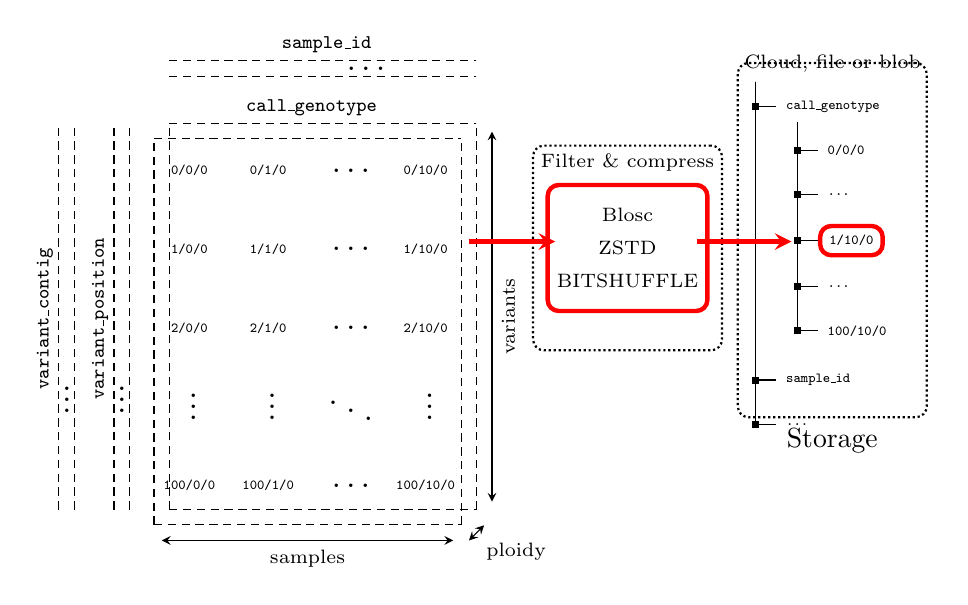
\begin{tikzpicture}


 %% sample_id
  \node at (2.0,5.9,-.5) {\ttfamily \scriptsize sample\textunderscore id};
  % bounds
  \draw[densely dashed] (0,5.5,-.5) -- (3.9,5.5,-.5);
  \draw[densely dashed] (0,5.7,-.5) -- (3.9,5.7,-.5);
 \tikzcuboidset{front face/.style={fill=yellow!20},right face/.style={fill=green!10},top face/.style={fill=yellow!20}}
  \pic at (0,5.5,-.5) {cuboid=.9--.2--0};
  \pic at (1,5.5,-.5) {cuboid=.9--.2--0};
  \node at (2.5,5.6,-.5) {\ttfamily \dots};
  \pic at (3,5.5,-.5) {cuboid=.9--.2--0};

 %% variant_contig
  \node[rotate=90] at (-1.5,2.5,-.3) {\ttfamily \scriptsize variant\textunderscore contig};
  % bounds
  \draw[densely dashed] (-1.4,0,-.5) -- (-1.4,4.9,-.5);
  \draw[densely dashed] (-1.2,0,-.5) -- (-1.2,4.9,-.5);
 \tikzcuboidset{front face/.style={fill=green!10},right face/.style={fill=green!10},top face/.style={fill=yellow!20}}
  \pic at (-1.4,0,-.5) {cuboid=.2--.9--0};
  \node at (-1.3,1.5,-.5) {\ttfamily \vdots};
  \pic at (-1.4,2,-.5) {cuboid=.2--.9--0};
  \pic at (-1.4,3,-.5) {cuboid=.2--.9--0};
  \pic at (-1.4,4,-.5) {cuboid=.2--.9--0};

 %% variant_position
  \node[rotate=90] at (-.8,2.5,-.3) {\ttfamily \scriptsize variant\textunderscore position};
  % bounds
  \draw[densely dashed] (-.7,0,-.5) -- (-.7,4.9,-.5);
  \draw[densely dashed] (-.5,0,-.5) -- (-.5,4.9,-.5);
 \tikzcuboidset{front face/.style={fill=green!10},right face/.style={fill=green!10},top face/.style={fill=yellow!20}}
  \pic at (-.7,0,-.5) {cuboid=.2--.9--0};
  \node at (-.6,1.5,-.5) {\ttfamily \vdots};
  \pic at (-.7,2,-.5) {cuboid=.2--.9--0};
  \pic at (-.7,3,-.5) {cuboid=.2--.9--0};
  \pic at (-.7,4,-.5) {cuboid=.2--.9--0};

 %% call_genotype
  \node at (2.0,5.3) {\ttfamily \scriptsize call\textunderscore genotype};
  % back box
  \draw[densely dashed] (0,0,-0.5) -- (3.9,0,-0.5);
  \draw[densely dashed] (0,0,-0.5) -- (0,4.9,-0.5);
  \draw[densely dashed] (0,4.9,-0.5) -- (3.9,4.9,-0.5);
  \draw[densely dashed] (3.9,0,-0.5) -- (3.9,4.9,-0.5);
 \tikzcuboidset{front face/.style={fill=blue!10},right face/.style={fill=green!10},top face/.style={fill=yellow!20}}
  \pic at (0,0) {cuboid=.9--.9--.5};
  \node at (0.45,0.5) {\ttfamily \tiny 100/0/0};
  \node at (0.5,1.6) {\ttfamily \vdots};
  \pic at (0,2) {cuboid=.9--.9--.5};
  \node at (0.45,2.5) {\ttfamily \tiny 2/0/0};
  \pic at (0,3) {cuboid=.9--.9--.5};
  \node at (0.45,3.5) {\ttfamily \tiny 1/0/0};
  \pic at (0,4) {cuboid=.9--.9--.5};
  \node at (0.45,4.5) {\ttfamily \tiny 0/0/0};
  \pic at (1,0) {cuboid=.9--.9--.5};
  \node at (1.45,0.5) {\ttfamily \tiny 100/1/0};
  \node at (1.5,1.6) {\ttfamily \vdots};
  \pic at (1,2) {cuboid=.9--.9--.5};
  \node at (1.45,2.5) {\ttfamily \tiny 2/1/0};
  \pic at (1,3) {cuboid=.9--.9--.5};
  \node at (1.45,3.5) {\ttfamily \tiny 1/1/0};
  \pic at (1,4) {cuboid=.9--.9--.5};
  \node at (1.45,4.5) {\ttfamily \tiny 0/1/0};
  \node at (2.5,0.5) {\ttfamily \dots};
  \node at (2.5,1.55) {\ttfamily $\ddots$};
  \node at (2.5,2.5) {\ttfamily \dots};
  \node at (2.5,3.5) {\ttfamily \dots};
  \node at (2.5,4.5) {\ttfamily \dots};
  \pic at (3,0) {cuboid=.9--.9--.5};
  \node at (3.45,0.5) {\ttfamily \tiny 100/10/0};
  \node at (3.5,1.6) {\ttfamily \vdots};
  \pic at (3,2) {cuboid=.9--.9--.5};
  \node at (3.45,2.5) {\ttfamily \tiny 2/10/0};
  \pic[ultra thick, red] at (3,3) {cuboid=.9--.9--.5};
  \node at (3.45,3.5) {\ttfamily \tiny 1/10/0};
  \pic at (3,4) {cuboid=.9--.9--.5};
  \node at (3.45,4.5) {\ttfamily \tiny 0/10/0};
  % front box
  \draw[densely dashed] (0,0) -- (3.9,0);
  \draw[densely dashed] (0,0) -- (0,4.9);
  \draw[densely dashed] (0,4.9) -- (3.9,4.9);
  \draw[densely dashed] (3.9,0) -- (3.9,4.9);
  
 %% dimensions
  \draw[stealth-stealth] (0.1,-0.2) -- (3.8,-0.2) node[midway,below] {\scriptsize samples};
  \draw[stealth-stealth] (4,-0.2, 0) -- (4,-0.2,-.5) node[midway,below right] {\scriptsize ploidy};
  \draw[stealth-stealth] (4.1,.1,-.5) -- (4.1,4.8,-.5) node[midway,below,rotate=90] {\scriptsize variants};

%% compresion
 \node (numcodecs) [rectangle, draw, densely dotted, thick, rounded corners, minimum width=2.4cm, minimum height=2.6cm, anchor= south west]
    at (4.8,2.2) {};
 \node[anchor=north,below] at (numcodecs.north) {\scriptsize Filter \& compress};
 %\node[anchor=south,below] at (numcodecs.south) {numcodecs};
 \node (blosk) [rectangle, ultra thick, red, draw, rounded corners, minimum width=1.8cm, minimum height=1.6cm, anchor=center,align=center,text=black]
    at (numcodecs) {\scriptsize Blosc\\\scriptsize ZSTD\\\scriptsize BITSHUFFLE};
 \draw[ultra thick, red,-stealth] (3.9,3.5,-.25) -- (5,3.5,-.25);

%% storage
 \node (location) [rectangle, draw, densely dotted, thick, rounded corners, minimum width=2.4cm, minimum height=4.5cm, anchor= south west]
    at (7.4,1.35) {};
 \node[anchor=south,below] at (location.south) {Storage};
 \node[anchor=center] at (location) {
        \begin{forest}
          for tree={
            font=\tiny ,
            grow'=0,
            child anchor=west,
            parent anchor=south,
            anchor=west,
            calign=first,
            edge path={
              \noexpand\path [draw, \forestoption{edge}]
              (!u.south west) +(7.5pt,0) |- node[fill,inner sep=1.25pt] {} (.child anchor)\forestoption{edge label};
            },
            before typesetting nodes={
              if n=1
                {insert before={[,phantom]}}
                {}
            },
            fit=band,
            before computing xy={l=15pt},
          }
        [{\scriptsize Cloud, file or blob}
          [\ttfamily call\textunderscore genotype
            [\ttfamily 0/0/0]
            [\ttfamily ...]
            [\ttfamily 1/10/0, draw={red,ultra thick, rounded corners}]
            [\ttfamily ...]
            [\ttfamily 100/10/0]
          ]
          [\ttfamily sample\textunderscore id]
          [\ttfamily ...]
        ]
        \end{forest}
 };
 \draw[ultra thick, red, -stealth,rounded corners=5pt] (6.8,3.5,-.25) -- (8,3.5,-.25);
 
\end{tikzpicture} 

}
\caption{Chunked compressed storage of VCF data using Zarr. 
The \texttt{call\_genotype} array is a three-dimensional (variants, samples,
ploidy) array of integers, split into a uniform grid of 
chunks determined by the variant and sample chunk sizes (10,000
and 1,000 by default in \texttt{vcf2zarr}). Each chunk is associated 
with a key defining its location in this grid, which can be stored 
in any key-value store such as a standard file-system or cloud object
store. Chunks are compressed independently using standard 
codecs and pre-compression filters, which can be specified on a per-array
basis. Also shown are the one-dimensional \texttt{variant\_contig} (CHROM)
and \texttt{variant\_position} arrays (POS). Other fields are stored 
in a similar fashion. \label{fig-data-model}}
\end{figure}

VCF is at its core an encoding of the genotype matrix, where each entry
describes the observed genotypes for a given sample at a given variant site,
interleaved with per-variant information
and other call-level matrices (e.g., the GQ or AD fields).
The data is largely numerical and of fixed dimension, 
and is therefore a natural mapping to array-oriented 
or ``tensor'' storage.
We propose the VCF Zarr specification which maps the 
VCF data model into an array-oriented layout using Zarr 
(Fig~\ref{fig-data-model}). 
In the VCF Zarr specification, 
each field in a VCF is mapped to an array, 
which is stored individually allowing for efficient retrieval and 
high levels of compression.
% In particular, call-level data is stored as $m \times n$ arrays
% (for $m$ sites and $n$ samples), allowing for efficient 
% retrieval of subsets of those fields along both the 
% variants and samples axis.
See the Methods for more detail on Zarr and the VCF Zarr
specification.

\begin{figure}
\begin{center}
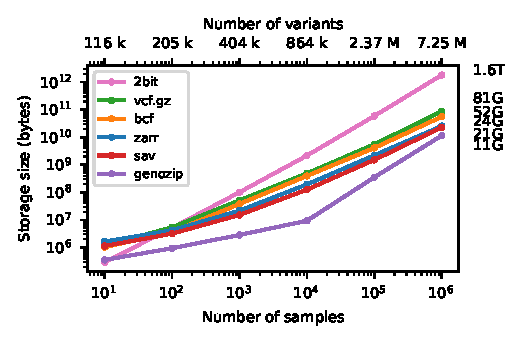
\includegraphics[]{figures/data-scaling}
\end{center}
\caption{Compression performance on simulated genotypes.
Comparison of total stored bytes for VCF data produced 
by subsets of a large simulation of French-Canadians.
Sizes for $10^6$ samples are shown on the right. Sizes 
for Savvy (21.25GiB) and Zarr (22.06GiB) are very similar.
Also shown for reference is the size of genotype matrix 
when encoded as two bits per diploid genotype (2bit), as used 
in the PLINK binary format.
\label{fig-data-storage}}
\end{figure}

One of the key benefits of Zarr is its cloud-native design, 
but it also works well on standard file systems, where 
arrays and chunks are stored hierarchically in directories
and files (storage as a single Zip archive is also supported).
To enable comparison with the existing file-based ecosystem
of tools, we focus on Zarr's file system chunk storage in a series of illustrative 
benchmarks in the following sections. 
(See \citep{durbin2020task,moore2021ome,gowan2022using} for Zarr
benchmarks in cloud settings.)
We compare primarily with
VCF/BCF based workflows using \texttt{bcftools} because this
is the standard practice, used in the vast majority of cases.
We also compare with two representative recent specialised utilities;
see~\cite{danek2018gtc,zhang2023gbc} for further benchmarks of 
these and other tools.
Genozip~\cite{lan2020genozip,lan2021genozip} is a tool focused 
on compression performance, which uses a custom file format 
and a CLI to extract VCF as text with various filtering options.
Savvy~\cite{lefaive2021sparse} is an extension of BCF which 
takes advantage of sparsity in the genotype matrix as well
as using PBWT-based approaches for improved compression.
Savvy provides a CLI as well as a C++ API.
Our benchmarks are based on genotype data 
from subsets of a large and highly realistic 
simulation of French-Canadians~\cite{anderson2023on}
(see Methods for details on the dataset and benchmarking methodology).
Note that while simulations cannot capture 
all the subtleties of real data, the allele frequency
and population structure patterns in this dataset 
have been shown to closely follow 
observations~\cite{anderson2023on} and so provides 
a reasonable and easily reproducible data point 
when comparing such methods.
The simulations only contain genotypes without any additional
high-entropy QC fields, which is unrealistic (see Section XXX
for benchmarks on a large human dataset that includes 
many such fields). 
Note, however, that such minimal, genotype-only data 
is something of a best-case scenario for specialised genotype
compression methods using row-based storage.

Fig~\ref{fig-data-storage} shows compression performance 
on up to a million samples for chromosome 21.
Unsurprisingly, gzip compressed VCF requires the most 
storage, with BCF providing substantially better compression
performance (note the log-log scale). Genozip has 
superb compression, having far smaller file sizes that the 
other methods (although somewhat losing its advantages at 
larger sample sizes). Zarr and Savvy have 
almost identical compression performance in this example.
It is remarkable that the simple approach of compressing
two dimensional chunks of the genotype matrix 
using the Zstandard compressor~\citep{collet2021rfc} and the 
bit-shuffle filter from Blosc~\cite{alted2010modern} produces 
compression levels competitive with the highly specialised methods
used by Savvy.

\subsection{Calculating with the genotype matrix}
Storing genetic variation data compactly is important, but it is also
important that we can analyse the data efficiently. Bioinformatics 
workflows tend to emphasise text files and command line utilities 
that consume and produce text~\citep[e.g.][]{buffalo2015bioinformatics}. 
Thus, many tools that compress VCF data provide a command line 
utility with a query language to restrict the records
examined, perform some pre-specified calculations and finally 
output some text, typically VCF or tab/comma separated values
[TODO check these citations]~\citep{
layer2016efficient, %GQT
li2016bgt, % BGT
tatwawadi2016gtrac, % GTRAC
danek2018gtc, % GTC
lin2020sparse, % SpVCF
lan2020genozip,lan2021genozip, %genozip
lefaive2021sparse, % SAVVY
wertenbroek2022xsi,% XSI
zhang2023gbc}. %GBC
These pre-defined calculations are by necessity limited in scope, however,
and the volumes of text involved in Biobank scale datasets
make the classical approach of custom
analyses via Unix utilities in pipelines prohibitively slow. Thus, 
methods have begun to provide Application Programming Interfaces
(APIs), providing efficient access to genotype and other VCF data
[TODO check these citations]~\cite[e.g.][]{kelleher2013processing,lefaive2021sparse,
wertenbroek2022xsi,zhang2023gbc}. By providing programmatic access,
the data can be retrieved from storage, decoded and then analysed
in the same memory space without additional copies and 
interprocess communication through pipes.

To demonstrate the accessibility of genotype data and efficiency with 
which calculations can be performed under the different formats,
we use the \texttt{bcftools +af-dist} plugin as an example.
% The details of the \texttt{af-dist} operation are not important:
% as an example of a whole-matrix operation. 
We chose this particular operation for several reasons. 
First, it is a straightforward calculation that 
requires examining every element in the genotype matrix,
and can be reproduced in different programming languages
without too much effort.
Secondly, it produces a small volume of output (a table of
deviations from Hardy-Weinberg expectations in ten allele frequency
bins) and therefore the time spent outputting results is negligible.
Finally, it has an efficient implementation written using the 
\texttt{htslib} C API~\citep{bonfield2021htslib}, distributed as 
a \texttt{bcftools} plugin. 

\begin{figure}
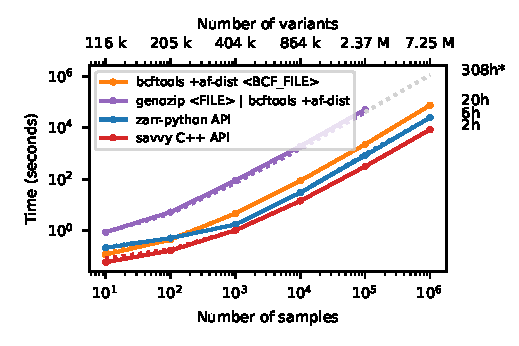
\includegraphics{figures/whole-matrix-compute}
\caption{Whole-matrix compute performance with increasing sample size.
Total CPU time required to run \texttt{bcftools +af-dist}
and equivalent operations in a single thread for various tools.
Elapsed time is also reported (dotted line). Run-time for genozip
and bcftools on VCF
at $10^6$ samples were extrapolated by fitting an exponential.
See Methods for full details.
\label{fig-whole-matrix-compute}}
\end{figure}

Fig~\ref{fig-whole-matrix-compute} shows timing results 
for running \texttt{bcftools +af-dist} and equivalent operations 
on the data of Fig~\ref{fig-data-storage}. There is a large
difference in the time required (note the log-log scale). 
The slowest approach uses Genozip. Because genozip does not
provide an API and only outputs VCF text, the best approach available 
is to pipe its output into \texttt{bcftools +af-dist}. Thus,
not only must we decode the data from the genozip format, we must 
then parse the large volumes of VCF text produced and then finally do the 
actual calculation. 
Running \texttt{bcftools +af-dist} directly on the gzipped VCF
is substantially faster, indicating that Genozip's excellent
compression performance comes at a substantial decompression cost.
Using a BCF file is again significantly faster,
because the packed binary format avoids the overhead of parsing 
VCF text into \texttt{htslib}'s internal data structures. 
We only use BCF for subsequent \texttt{bcftools} benchmarks.

The data shown in Fig~\ref{fig-whole-matrix-compute} for Zarr and Savvy
is based on custom programs written using their respective APIs
to implement the \texttt{af-dist} operation. The Zarr program uses
the Zarr-Python package to iterate over the decoded chunks of the 
genotype matrix and classifies genotypes within a chunk using a 14 line Python
function, accelerated using the Numba JIT compliler~\cite{lam2015numba}.
The allele frequencies and genotype counts are then analysed to produce 
the final counts within the allele frequency bins with 9 lines of 
Python using NumPy~\cite{harris2020array} functions. Remarkably, this 
short and simple Python program is substantially faster than the 
equivalent compiled C using \texttt{htslib} APIs on BCF (6.9 hours
vs 20.6 hours for 1 million samples). 
% num_samples  num_sites      tool  user_time  sys_time     wall_time  total_time
%     1000000    7254858     savvy    8371.07      4.16   8377.718136  2.326453
%     1000000    7254858  bcftools   73939.32     46.09  74023.083678  20.551503
%     1000000    7254858      zarr   24709.64     29.32  24750.704171  6.871933
The fastest method is the 
C++ program written using the Savvy API. This would largely seem
to be due to Savvy's excellent genotype decoding performance
% zarr 1.2 GiB
% savvy 6.6 GiB
% zarr_nshf 3.9 GiB
(up to 6.6GiB/s vs 1.2GiB/s for Zarr on this dataset;
Fig~\ref{fig-whole-matrix-decode}).
% sequence_length  num_samples  num_sites       tool       size
% 40         48129895      1000000    7254858       zarr  22.071687
% 35         48129895      1000000    7254858        bcf  51.749294
% 36         48129895      1000000    7254858    genozip  10.691384
% 37         48129895      1000000    7254858        sav  21.249436
% 38         48129895      1000000    7254858        tsk   1.802636
% 39         48129895      1000000    7254858        vcf  81.375831
% 41         48129895      1000000    7254858  zarr_nshf  29.897540
Turning off the BitShuffle filter for the Zarr dataset,
however, leads to a substantial increase in decoding speed
(3.9GiB/s) at the cost of a roughly 25\% increase in storage
space (29.9GiB up from 22.1GiB for 1 million samples; data not
shown). Given the relatively small contribution of genotypes to the
overall storage of real datasets (see the Genomics England example)
and the frequency that they are likely to be accessed, this
would seem like a good tradeoff in most cases.
This ability to easily tune compression performance
and decoding speed on a field-by-field basis is a major strong
point of Zarr. The \texttt{vcf2zarr} utility also provides
functionality to aid with such storage schema tuning.


\subsection{Subsetting the genotype matrix}
As datasets grow ever larger, the ability to efficiently access subsets 
of the data becomes more and more important. VCF/BCF achieve efficient 
access to the data for genomic ranges 
by compressing blocks of adjacent records using \texttt{bgzip},
and storing secondary indexes alongside the original 
files with a conventional suffix~\citep{li2011tabix}. 
Thus, for a given range query we 
decompress only the necessary blocks and can quickly access
the required records. 
Methods like Savvy and XSI largely follow the same principles [TODO check and 
be more concrete]. The row-wise nature of these methods, however, mean 
that we cannot efficiently subset \emph{by sample}
(e.g., to calculate statistics within a particular cohort). In the extreme
case, if we want to access only the genotypes for a single sample
we must still retrieve and decompress the entire dataset.

\begin{figure}
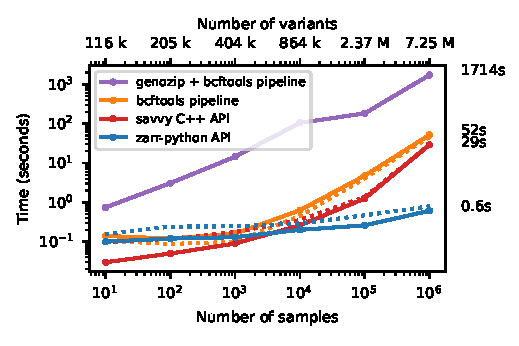
\includegraphics{figures/subset-matrix-compute}
\caption{Compute performance on subsets of the matrix.
Total CPU time required to run the af-dist calculation for
a subset of 10000 variants $\times$ 10 samples from the middle of the matrix
for the data in Fig~\ref{fig-data-storage}.
The \texttt{genozip} and \texttt{bcftools} pipelines involve
multiple commands required to correctly calculate the AF INFO field
required by \texttt{bcftools +af-dist}. See the Methods for full details
on the steps performed.
\label{fig-subset-matrix-compute}}
\end{figure}

We illustrate the cost of row-wise encoding in
Fig~\ref{fig-subset-matrix-compute}, where we run the af-dist calculation
on a small fixed-size subset of the genotype matrices of
Fig~\ref{fig-data-storage}. The two-dimensional chunking of Zarr
means that this small subset of the overall matrix can be efficiently
extracted, and therefore the execution time depends very weakly on 
the overall dataset size, with the overall computation requiring around
1 second for 1 million samples. Because of their 
row-wise encoding for all the other methods CPU time
scales with the number of samples.
Fig~\ref{fig-subset-matrix-compute-supplemental} shows performance
for the same operation when selecting half of the samples in the 
dataset.

\begin{figure}
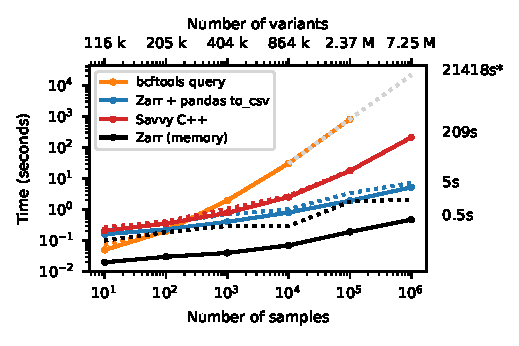
\includegraphics{figures/column-extract}
\caption{Time to extract the genome position and write to a text file.
Total CPU time required to extract the POS field for BCF,
sav and Zarr formats
for the data in Figure~\ref{fig-data-storage}.
For the BCF file we used \texttt{bcftools query -f"\%POS$\backslash$n"}.
For sav, we used the Savvy C++ API to extract just the position, 
and output text using the \texttt{std::cout} stream. For Zarr, we read 
\texttt{variant\_position} into a NumPy array, and then wrote to
a text file using the Pandas \texttt{write\_csv} method. 
Zarr CPU time is dominated by writing the text output; we also show
the time required to populate a NumPy array with the data in Zarr,
which is less than a second. Wall-clock time (dotted line) is dominated 
in this case by file I/O. Time to output text for Savvy is not significant
for $> 1000$ samples (not shown).
\label{fig-column-extract}}
\end{figure}

\subsection{Extracting fields}
We have focused on the genotype matrix up to this point, contrasting
Zarr with existing row-wise methods.
Real-world VCFs encapsulate much more than just the genotype
matrix, and can contain large numbers of additional fields.
Fig~\ref{fig-column-extract} shows the time required to extract 
the genomic position of each variant in the simulated benchmark 
dataset, which we can use as an indicative example of a per-variant 
query. Although Savvy is many times faster than \texttt{bcftools query}
here, the row-wise storage strategy that they share means that 
the entire dataset must be read into memory and 
decompressed to extract just one field from each record. Zarr
excels at these tasks: we only read and decompress the information required.

\subsection{Case study: Genomics England 100,000 genomes}
In this section we demonstrate the utility of VCF Zarr on a large human dataset
and the scalability of the \texttt{vcf2zarr} conversion utility.
Genomics England’s multi-sample VCF dataset (aggV2) is an 
aggregate of 78,195 gVCFs from rare disease and cancer participants 
recruited as part of the 100,000 Genomes Project~\cite{turnbull2018100}. 
The dataset comprises approximately 722 million annotated single-nucleotide 
variants (SNVs) and small indels split into 1,371 roughly equal chunks and 
totalling 165.3 TiB of VCF data after \texttt{bgzip} compression. 
The dataset is used for a variety of research purposes, ranging from 
genome-wide association studies (GWAS)~\cite{kousathanas2022whole} and 
imputation~\cite{shi2023genomics} to 
simple queries involving single gene 
regions~\cite{leggatt2023genotype,lam2023repeat}.

As described in the Methods, conversion to Zarr using 
\texttt{vcf2zarr} is a two-step 
process to limit memory usage and ensure reliability. We 
first converted the 28 VCF files (3.51 TiB) for chromosome 20
into the intermediate columnar format (ICF). This task was 
split into 3899 partitions, and distributed using the Genomics England
HPC cluster. It required about 50 days of CPU, with an elapsed
wall-clock time of about 2 hours. The ICF representation uses a total
of XTiB over XX files and YY directories. We then encoded this intermediate
columnar format to Zarr using 8 cores and XX GB of RAM in about 12 hours.
This produced a dataset with 43 arrays, consuming a 
total of Y GiB of storage over X directories and 
Y files. This is about a 4.8X reduction over the original VCF. 
The top fields in terms 
of storage are detailed in Table~\ref{tab-genomics-england-data}.

\begin{table}
\caption{Summary for a selection of the largest VCF Zarr columns produced for 
Genomics England aggV2 VCFs on chromosome 20 using \texttt{vcf2zarr}
default settings. Each field is stored independently 
as a Zarr array with the given type (sufficient to represent all values in the
data). We show the total storage consumed (reported via \texttt{du}) in 
power-of-two units, and the compression ratio achieved on that array.
We also show the percentage of the overall storage that each array consumes.
\label{tab-genomics-england-data}}
\begin{tabular}{llS[table-format=3.1]S[table-format=3.2]S[table-format=3.2]}
\toprule
{Field} & {type} & {storage} & {compress} & {\%total} \\
\midrule
call\_AD &  int16 & 179.7G & 26 & 24.0\\
call\_GQ &  int16 & 171.8G & 13 & 23.0 \\
call\_DP &  int16 & 141.8G & 16 & 18.9 \\
call\_DPF& int16  & 115.1G & 20 & 15.3\\
call\_FT &  string & 58.5G & 160 & 7.8 \\
call\_PL &  int16 & 51.4G & 140 & 6.9 \\
call\_GQX &  int16 & 12.1G & 190 & 1.6 \\
call\_genotype & int8 & 6.1G & 380 & 0.8 \\
call\_genotype\_mask & bool & 3.7G  & 630 & 0.5\\
call\_genotype\_phased & bool & 692.5M  & 1700 & 0.1 \\
call\_PS  & int8  & 102.2M & 12000 & 0.05 \\
variant\_quality & float32 & 22.6M & 2.7 & <0.01 \\
variant\_allele & string & 21.5M & 11 \\
variant\_position & int32 & 12.7M & 4.7 \\
variant\_ABratio & float32 & 9.6M & 6.3 \\
variant\_AN & int32 & 9.6M & 6.3 \\
variant\_filter & bool & 1.9M & 490 \\
\bottomrule
\end{tabular}
\end{table}

% array([23.956     , 22.90533333, 18.90133333, 15.34533333,  7.8       ,
%         6.85333333,  1.61066667,  0.81733333,  0.488     ])

% /call_AD                     int16    179.67 GiB  4.53 TiB       26 125768  37.74 MiB     1.46 MiB            (15912293, 78195, 2)  (10000, 1000, 2)  
% /call_GQ                     int16    171.79 GiB  2.26 TiB       13 125768  18.87 MiB     1.4 MiB             (15912293, 78195)     (10000, 1000) 
% /call_DP                     int16    141.76 GiB  2.26 TiB       16 125768  18.87 MiB     1.15 MiB            (15912293, 78195)     (10000, 1000)
% /call_DPF                    int16    115.09 GiB  2.26 TiB       20 125768  18.87 MiB     959.56 KiB          (15912293, 78195)     (10000, 1000)
% /call_FT                     object   58.5 GiB    9.05 TiB      160 125768  75.48 MiB     487.71 KiB          (15912293, 78195)     (10000, 1000)
% /call_PL                     int16    51.4 GiB    6.79 TiB      140 125768  56.61 MiB     428.51 KiB          (15912293, 78195, 3)  (10000, 1000, 3)
% /call_GQX                    int16    12.08 GiB   2.26 TiB      190 125768  18.87 MiB     100.73 KiB          (15912293, 78195)     (10000, 1000) 
% /call_genotype               int8     6.13 GiB    2.26 TiB      380 125768  18.87 MiB     51.11 KiB           (15912293, 78195, 2)  (10000, 1000, 2)  
% /call_genotype_mask          bool     3.66 GiB    2.26 TiB      630 125768  18.87 MiB     30.53 KiB           (15912293, 78195, 2)  (10000, 1000, 2)  
% /call_genotype_phased        bool     692.51 MiB  1.13 TiB     1700 125768  9.43 MiB      5.64 KiB            (15912293, 78195)     (10000, 1000) 
% /call_PS                     int8     102.2 MiB   1.13 TiB    12000 125768  9.43 MiB      852 bytes           (15912293, 78195)     (10000, 1000) 
% /call_ADR                    int8     102.2 MiB   1.13 TiB    12000 125768  9.43 MiB      852 bytes           (15912293, 78195)     (10000, 1000)
% /call_ADF                    int8     102.2 MiB   1.13 TiB    12000 125768  9.43 MiB      852 bytes           (15912293, 78195)     (10000, 1000)
% /variant_OLD_MULTIALLELIC    object   31.63 MiB   121.4 MiB       3.8 1592  78.09 KiB     20.34 KiB           (15912293,)           (10000,) 
% /variant_quality             float32  22.6 MiB    60.7 MiB        2.7 1592  39.04 KiB     14.53 KiB           (15912293,)           (10000,) 
% /variant_allele              object   21.52 MiB   242.8 MiB      11 1592  156.17 KiB    13.84 KiB           (15912293, 2)         (10000, 2) 
% /variant_position            int32    12.83 MiB   60.7 MiB        4.7 1592  39.04 KiB     8.25 KiB            (15912293,)           (10000,) 
% /variant_ABratio             float32  9.62 MiB    60.7 MiB        6.3 1592  39.04 KiB     6.18 KiB            (15912293,)           (10000,) 
% /variant_AN                  int32    9.6 MiB     60.7 MiB        6.3 1592  39.04 KiB     6.18 KiB            (15912293,)           (10000,) 
% /variant_AC                  int32    9.22 MiB    60.7 MiB        6.6 1592  39.04 KiB     5.93 KiB            (15912293,)           (10000,) 
% /variant_AC_Het              int32    8.98 MiB    60.7 MiB        6.8 1592  39.04 KiB     5.78 KiB            (15912293,)           (10000,) 

% Approx total = 179.67 + 171.79 + 141.76 + 115.09 + 58.5 + 51.4 + 12.08 + 6.13 + 3.66 
% 740, round up to 750
% [179.67 , 171.79 , 141.76 , 115.09 , 58.5 , 51.4 , 12.08 , 6.13 , 3.66 ]
% >>> import numpy as np
% >>> a = np.array([179.67 , 171.79 , 141.76 , 115.09 , 58.5 , 51.4 , 12.08 ,
% 6.13 , 3.66 ]  )
% >>> a
% array([179.67, 171.79, 141.76, 115.09,  58.5 ,  51.4 ,  12.08,   6.13,
%          3.66])
% >>> a / 750 * 100
% array([23.956     , 22.90533333, 18.90133333, 15.34533333,  7.8       ,
%         6.85333333,  1.61066667,  0.81733333,  0.488     ])

Table~\ref{tab-genomics-england-data} shows that the dataset storage
size is dominated by a few columns with the top four
(call\_AD, call\_GQ, call\_DP and call\_DPF) accounting for over 
80\% of the total. These fields are much less compressible
than genotype data (which uses $<1\%$ of the total space here)
because of their inherent noisiness~\citep{lin2020sparse}. 

[TODO add in benchmarks discussed in issue. Extract POS, run af-dist, 
do a filtering query. Note problems with orchestration when
dealing with multiple VCF chunks. 
Talk about mask-oriented computing there at the
end, pointing out the cost of these multiple copies.]

% By default the \texttt{bio2zarr} conversion is lossless, and integers
% of the narrowest type required to represent all of the data are
% used. In this case, this has resulted in 16 bit integers being used 
% for these top four fields. Examining the distribution of the depth
% fields, (call\_AD, call\_DP, call\_DPF), we can 
% we can see that a tiny fraction of the values stored
% are greater than 127 (call\_AD: 0.1\%, call\_DP: xx\%, call\_DPF: x\%; see 
% Fig SX for histograms).
% One might then reasonably truncate these fields to 8 bit integers.
% After converting to 8 bit, call\_AD is reduced by 
% x\% (XX GiB) and call\_DP reduced by x\% (XX GiB)
% and call\_DPF by x\% (XX GiB). 
% Similarly, the vast majority of call\_GQ values (xx\%) are less than 
% 128 (corresponding to a conditional probability that the genotype call is 
% wrong of $10^{-128}$ [TODO CHECK THIS]), and can also reasonably
% be truncated. Here, this results in a reduction of x\% (XX GiB).
% Combined, truncating these top four fields to 8 bits reduces the 
% overall storage of the dataset to XXGiB, corresponding to a 
% X-fold compression of the VCF.

% and can reasonably be truncated (a 
% much information would be lost if we used 8 bit
% Substantial
% reductions in space can be achieved, however, if we examine the 
% distributions of these fields and truncate some outliers.
% Figure~SX shows the histogram of the XX call\_AD values, and we can
% see that < 0.0X\% of the values are $>127$. Truncating and 
% re-encoding the call\_AD array as an int8 results in a total storage of 
% XX. A substantial advantage of Zarr is that such per-field optimisations
% can be made after conversion, without affecting the rest of the dataset.
% As discussed in Methods, judicious use of additional filters
% and lossy quantizing can result substantial space savings.

% Calculating the histogram of per call values at this 
% scale is not a trivial task.
% Taking advantage of the rich software ecosystem growing around Zarr
% (see Discussion) we used xarray~\citep{hoyer2017xarray}
% and Dask~\citep{rocklin2015dask} to transparently distribute the 
% computations over a cluster of X workers. 
% [ADD DETAILS]
% The elapsed time was X minutes, and requires X lines of Python in a 
% Jupyter notebook~\citep{kluyver2016jupyter}. 

% One of the key uses of the aggV2 dataset is to enable simple queries 
% of specific regions. For example, in [A PAPER] they [DID SOMETHING].
% We replicated this by running the appropriate bcftools query
% on the VCF chunk (note that the user is responsible for finding 
% the correct chunk file here, limiting the utility of genomic 
% indexes). This took XXX hours.
% The same query implemented with the Zarr-python 
% API required XXX seconds to produce identical output.

\section{Discussion}
% Zarr is great
VCF is a central element of modern genomics, facilitating
the exchange of data among interoperating tools. 
Its current row-oriented form, however,
is fundamentally inefficient,
profoundly limiting the scalability of the current generation
of bioinformatics tools. Large scale VCF data cannot 
currently be 
processed without incurring a substantial economic
and likely environmental cost~\cite{grealey2022carbon}.
We have shown here that this is not a necessary situation,
and that greatly improved efficiency can be achieved by 
using more appropriate storage representations tuned
to the realities of modern computing. We have argued that 
Zarr provides a powerful basis for cloud-based
storage and analysis of large-scale genetic variation data.
We propose the VCF Zarr specification which losslessly
maps VCF data to Zarr, and provide an efficient and scalable
tool to perform conversion.

% We're not pretending is a solution to all problems and
% up front about weaknesses of the model.
Zarr provides pragmatic solutions to some of the more pressing 
problems facing the analysis of large-scale genetic variation
data, but it is not a solution to all problems. Firstly, 
any dataset containing a variant with a large number of alleles
(perhaps due to indels) will cause problems because the 
dimensions of various fields are determined by the \emph{maximum}
dimension among all variants. Secondly, the design of 
VCF Zarr emphasises efficiency of analysis for a fixed 
dataset, and does not consider problems of ongoing updates
(i.e, as new samples and their variants are added).
Thirdly, Zarr is not suitable for handling unstructured
string data, and for example likely not work well as a 
basis for storing annotation data [CITES].

Nonetheless, there are numerous datasets that exist today
what would benefit from cloud-native storage, 
inherent parallelism and granular storage.
[Mention benefits of fine-grained access control to 
different parts of the dataset using native storage access
control mechanism?]

The VCF Zarr specification and scalable vcf2zarr conversion utility
that we have provided here are the starting points of such 
an ecosystem, but much more would be needed to make a viable 
alternative for everyday bioinformatics workflows. However, a few key
pieces of infrastructure would provide a starting point, and would 
be sufficient to greatly improve researcher productivity on 
large, centrally managed datasets such as Genomics England.
Firstly, a \texttt{vcfzarrtools} command line utility which 
implements a subset of \texttt{bcftools} functionality (such as 
\texttt{view} and \texttt{query}) would immediately speed up 
limited region and field specific queries by orders of magnitude,
and would provide compatibility with existing workflows.
Developing such a utility would be a non-trivial but routine
engineering task.

The second key piece of infrastructure required at this large 
scale concerns distributed computation. Even with more efficient
columnar data representations, computations that required examing 
large volumes of per-call data must be distributed to complete 
in a reasonable amount of time. [Dask, Xarray, sgkit?]


% \item Vision. An ecosystem of tools that interoperate
% based on an open, cloud-based format where distribution is naturally
% managed by the stored chunks. Tools can be run on different datasets
% with minimal tuning, not by writing a full layer of orchestration.
% Tools read the data they need, not the entire dataset. Users read
% directly from a single canonical dataset, and do not maintain
% their own filtered copies. We suggest that the Zarr VCF approach
% we have provided would be a good starting point for designing
% such a compute platform.

% \end{itemize}

The Python data science ecosystem, 
built on the foundations of efficient array-oriented 
computing~\citep{harris2020array},
has a rich suite of powerful tools~\cite{
mckinney2010data,
rocklin2015dask,
kluyver2016jupyter,
hoyer2017xarray,
virtanen2020scipy} and gaining increasing
popularity in recent biological applications~\citep[e.g.][]{
abdennur2020cooler,
rand2022bionumpy,
open2c2024bioframe,
hou2024admix}.
Zarr has the potential to act as a unified, cloud-native 
efficient storage layer, freeing the next generation of 
bioinformatics tools
from the traditional burdens of text parsing and format
conversion.

\section{Methods}

\subsection{Zarr and block-based compression}
% Zarr is a simple layer on top of best-in-class, modern components
In the interest of completeness it is useful to provide a high-level overview
of Zarr and the techologies that it depends upon. Zarr is a specialised format
for storing large-scale $n$-dimensional data (arrays). Arrays
are split into chunks, which are compressed and stored separately. Chunks are 
addressed by their indexes along the dimensions of the array, and the 
compressed data associated with this key. Chunks can
be stored in individual files (as we do here), but a wide array of different
storage backends are supported including cloud object stores 
and NoSQL databases;
in principle, Zarr can store data in any key-value store.
Metadata describing the array and its properties is then stored 
in JSON format along with the chunks. The simplicity and transparency
of this design has substantial advantages over other technologies
such as HDF5~\citep{folk2011overview} which are relatively complex and opaque.
This simplicity has led to numerous implementations of the Zarr specification
being developed, ranging from the mature Zarr-Python~\citep{zarrpython}
and TensorStore~\citep{tensorstore} implementations
to more experimental extensions to packages like
GDAL~\citep{gdal_zarr},
NetCDF~\citep{netcfd_c},
N5~\citep{n5zarr}
and xtensor~\citep{xtensor_zarr}
as well as  standalone libraries for JavaScript~\cite{zarrjs},
Julia~\cite{zarrjl}, Rust~\citep{zarrs}
and R~\cite{pizzarr}.

Zarr is flexible in allowing different compression codecs and 
pre-compression filters to be specified on a per-array basis
(see section XXX).
Two key technologies often used in conjunction with Zarr are the Blosc
% This seems like the best citation for Blosc? It is mentioned here
meta-compressor~\cite{alted2010modern}
and Zstandard compression algorithm~\citep{collet2021rfc}.
Blosc is a high-performance compressor optimised for numerical
data which uses ``blocking''~\citep{alted2010modern} to 
optimise CPU-cache access patterns, as well as highly optimised
bit and byte shuffle filters.  Remarkably, on highly 
compressible datasets, Blosc decompression can be faster 
than \texttt{memcpy}.
% Mentioning this detail to reassure readers who might be thinking
% "how would this be implemented and what kind of horrible dependencies
% would I need?"
Blosc is written in C, with APIs for C, Python, Julia, Rust
and others.
Blosc is a ``meta-compressor'' because it provides 
access to several different compression codecs. The 
Zstandard codec is of particular 
interest here as it achieves very high compression ratios
with good decompression speeds. See Fig~\ref{fig-whole-matrix-decode}
for a comparison of Zstandard with LZ4 on decoding performance.
% This may seem a bit off topic, but want to reassure reader that 
% this isn't some niche technology
Zstandard is also used in several recent VCF compression 
methods~\citep[e.g.][]{lefaive2021sparse,wertenbroek2022xsi}.
% LZ4 is also notable - any citations for this?

Scientific datasets are increasingly overwhelming the classical
model of downloading and analysing locally, and are migrating to 
centralised cloud repositories \citep{abernathey2021cloud,moore2021ome}.
The combination of Zarr's simple and cloud-friendly storage 
of data chunks with state-of-the-art compression methods has 
led to Zarr gaining significant traction in these settings.
Multiple petabyte-scale datasets are now stored using 
Zarr~\cite[e.g.][]{gowan2022using, % weather model data
fahnestock2023mappin, % ITS_LIVE dataset
cmip6_dataset}
or under active consideration for migration~\citep{durbin2020task,abernathey2021opening}.
The Open GeoSpatial consortium has formally recognised Zarr as a community
standard~\cite{ogc_zarr2_standard}
and has formed
a new GeoZarr Standards Working Group to establish a Zarr encoding for
geospatial data~\cite{ogc_geozarr_news}.

Zarr has recently been gaining popularity in biological applications.
The Open Microscopy Environment has developed OME-Zarr~\cite{moore2023ome} as one 
of its ``next generation'' cloud ready file formats~\citep{moore2021ome}.
OME-Zarr already has a rich suite of supporting
tools~\cite{moore2023ome,rzepka2023toward}. 
Zarr has also seen recent uptake 
in single-cell single-cell genomics~\citep{dhapola2022scarf,virshup2023scverse}
and multimodal spatial omics
data~\citep{marconato2024spatialdata,baker2023emobject}.
Recent additions using Zarr include the application of deep learning
models to genomic sequence data~\citep{klie2023predictive} 
and a browser for genetic variation data~\citep{konig2023divbrowse}.
Zarr has in fact been in use in genomics for many years, and was originally 
developed to [ALISTAIR - details and citations here!]

\subsection{The VCF Zarr specification}
The VCF Zarr specification is a direct mapping from the VCF data model
to a chunked binary array format using Zarr. VCF Zarr takes advantage
of Zarr's hierarchical structure by representing a VCF file as a top-level
Zarr group containing Zarr arrays. Each VCF field (fixed fields, INFO fields,
and FORMAT fields) is represented as a separate array in the Zarr hierarchy.
Some of the structures from the VCF header are also represented as arrays,
including contigs, filters, and samples.

% Do we need to say that VCF Zarr is an evolution of the Zarr format in scikit-allel?

The specification defines the name, shape, dimension names, and data type
for each array in the Zarr store. These ``logical'' properties are mandated,
in contrast to ``physical'' Zarr array properties such as chunk sizes and
compression, which can be freely chosen by the implementation. This
separation makes it straightforward for tools and applications to consume
VCF Zarr data since the data has a well-defined structure, while allowing
implementations enough room to optimise chunk sizes and compression
according to the application's needs.

The specification defines a clear mapping of VCF field names (keys) to
array names, VCF Number to array shape, and VCF Type to array data type.
To take one example, consider the VCF AD genotype field defined by the
following VCF header: \texttt{
\#\#FORMAT=<ID=AD,Number=A,Type=Integer,Description="Allele Depths">}.
The FORMAT key \texttt{ID} maps to an array name of \texttt{call\_AD}
(FORMAT fields have a \texttt{call\_} prefix, while INFO fields have a
\texttt{variant\_} prefix; both are followed by the key name). Arrays
corresponding to FORMAT fields are 3-dimensional with shapes that look
like \texttt{(variants, samples, <Number>)} in general. In this case, the
Number A entry indicates that the field has one value per alternate allele,
which in VCF Zarr is represented as the \texttt{alt\_alleles} dimension name,
so the shape of this array is \texttt{(variants, samples, alt\_alleles)}.
The VCF Integer type can be represented as any Zarr integer type, 
and the specification doesn't mandate particular integer widths. 
The \texttt{vcf2zarr} (see the next section) conversion utility 
chooses the narrowest integer width that can represent the data in
each field.

An important aspect of VCF Zarr is that field dimensions are 
global and fixed, and defined as the maximum across all rows.
Continuing the example above, the third dimension of the array 
is the maximum number of alternate alleles across \emph{all} 
variants. For variants at which there are less than the maximum
number of alternative alleles, the third dimension of the 
\texttt{call\_AD} array
is padded with a sentinel value (-2 for integers and a specific
non-signalling NaN for floats). While this is not a problem 
in practise for datasets in which all four bases are observed, 
it is a substantial issue for
fields that have a quadratic dependency on the number of alleles
(Number=G) such as PL. Such fields are already known to cause 
significant problems, and the ``local alleles'' proposal 
provides an elegant solution~\cite{poterba2024scalable}.
As this approach is on a likely path to 
standardisation~\cite{danecek2021twelve}, we would aim to 
include support in later versions of VCF Zarr.

The VCF Zarr specification can represent anything described by BCF
(which is somewhat more restrictive than VCF) except for two corner
cases related to the encoding of missing data. Firstly, VCF Zarr does
not distinguish between a field that is not present and one that 
is present but contains missing data. For example, a variant with an
INFO field \texttt{NS=.} is represented in the same way in VCF Zarr
as an INFO field with no \texttt{NS} key. Secondly, because of the use
of sentinel values to represent missing and fill values for integers
(-1 and -2, respectively), a field containing these original values
cannot be stored. In practice this doesn't seem to be much of 
an issue (we have not found a real VCF that contains negative 
integers). However, if -1 and -2 need to be stored, a float field
can be used without issues.

The VCF Zarr specification is general and can be mapped to 
file formats such as \toolname{plink}~\citep{purcell2007plink,chang2015second}
and BGEN~\citep{band2018bgen} with some minor extensions.

\subsection{vcf2zarr}
Converting VCF to Zarr at Biobank scale is challenging. 
One problem is to determine the dimension of fields,
(i.e., finding the maximum number of alternate alleles and the 
maximum size of \texttt{Number=.} fields) which requires a full
pass through the data. Another challenge is to keep
memory usage within reasonable limits: although 
we can view each record in the VCF one-by-one,
we must buffer a full chunk (10,000 variants is the default in
\texttt{vcf2zarr}) 
in the variants dimension for each of the fields to convert to Zarr. 
For VCFs with many FORMAT fields and large numbers of samples this can
require tens of gigabytes of RAM per worker, making
parallelism difficult. Reading the VCF multiple times for different fields
is possible, but would be prohibitively slow for multi-terabyte VCFs.

The \texttt{vcf2zarr} utility solves this problem by first converting 
the VCF data (which can be split across many files) into an Intermediate
Columnar Format (ICF). The \texttt{vcf2zarr explode} command takes a set
of VCFs, and reads through them using
\texttt{cyvcf2}~\cite{pedersen2017cyvcf2},
storing each field independently in (approximately) fixed-size 
compressed chunks.
Large files can be partitioned based on information extracted from the 
CSI or Tabix indexes, and so different parts of a file can be 
converted to ICF in parallel.
Once all partitions have completed, information about 
the number of records in each partition and chunk of a given
field is stored so that the record at a particular index 
can be efficiently retrieved. 
Summaries such as maximum dimension and the minimum and maximum value 
of each field are also maintained, to aid choice of data types later.
A set of VCF files can be converted to intermediate columnar 
format in parallel on a single machine 
using the \texttt{explode} command,
or can be distributed across a cluster using the 
\texttt{dexplode-init},
\texttt{dexplode-partition} and \texttt{dexplode-finalise} commands.

Once the VCF data has been converted to the intermediate columnar format,
it can then be converted to Zarr using the \texttt{vcf2zarr encode}
command. We take advantage of Zarr's flexibility
in \texttt{vcf2zarr} by choosing integer widths based 

and reasonable compressor defaults, but these can be
modified by generating and editing a JSON-formatted storage schema.
Encoding a given column (for example, \texttt{call\_AD})
involves creating a buffer to hold a full variant-chunk of the 
array in question, and then sequentially filling this buffer with 
values read from ICF and flushing to file. Similar to the \texttt{explode} command,
encoding to Zarr can be done in parallel on a single 
machine using the \texttt{encode} command,
or can be distributed across a cluster using the 
\texttt{dencode-init},
\texttt{dencode-partition} and \texttt{dencode-finalise} commands.
The distributed commands are fault-tolerant, reporting any failed
parititions so that they can be retried.

\subsection{Choosing default compressor settings}
To inform the choice of compression settings across different fields 
in VCF data, we analysed their effect on compression ratio on 
data from the 1000 Genomes project.
[TODO, reffing Fig~\ref{fig-compression-shuffle} and 
Fig~\ref{fig-compression-chunksize}.]

% [FILL IN WITH Shadi's analysis from here:
% https://github.com/sgkit-dev/bio2zarr/discussions/74
% Discussed in:
% https://github.com/sgkit-dev/vcf-zarr-publication/issues/26

\subsection{Benchmarks}
In this section we describe the methodology used for the simulation-based
benchmarks of Figs~\ref{fig-data-storage},\ref{fig-whole-matrix-compute},
\ref{fig-subset-matrix-compute} and \ref{fig-column-extract}.
The benchmarks use data simulated by conditioning on a large
pedigree of French-Canadians using 
\texttt{msprime}~\citep{baumdicker2021efficient},
which have been shown to follow patterns observed in real 
data from the same population to a remarkable 
degree~\cite{anderson2023on}.
We begin by downloading the simulated ancestral recombination 
graph~\cite{brandt2024promise,lewanski2024era,wong2024general}
for chromosome 21 from Zenodo~\cite{anderson2023simulated} 
in compressed \texttt{tszip} format. This 552M file 
contains the simulated ancestry and mutations for 1.4 million
present-day samples. We then subset the full simulation 
down to ${10^1, 10^2, \dots, 10^6}$ samples using 
ARG simplification~\cite{kelleher2018efficient,wong2024general},
storing the subsets in \texttt{tskit} format~\cite{tskit2024}.
Note that this procedure captures the growth 
in the number of variants (shown in the top x-axis labels)
as we increase sample sizes as a 
natural consequence of population-genetic processes.
% jk@holly$ python3 src/collect_data.py site-allele-report
% scaling/data/chr21_10_6.zarr/
% 0 alleles:  100.00%
% 1 alleles:  100.00%
% 2 alleles:  7.92%
% 3 alleles:  0.21%
As a result of simulated mutational processes,
most sites have one alternate allele, 
with 7.9\% having two and 0.2\% having three
alternate alleles in the $10^6$ samples dataset.
We then export the variation data from each subset to VCF
using \texttt{tskit vcf subset.ts | bgzip > subset.vcf.gz}
as the starting point for other tools.

We used bcftools version 1.18, Savvy 2.1.0, Genozip 5.0.26,
vcf2zarr 0.0.9, and Zarr-Python 2.17.2. 
All tools used default settings, 
unless otherwise stated.
All simulation-based benchmarks were performed on a 
dual CPU (Intel Xeon E5-2680 v2)
server with 256GiB of RAM running Debian GNU/Linux 11.
To ensure that the true effects of having data distributed over a large 
number of files were reported, benchmarks for Zarr and Savvy were 
performed on a cold disk cache by running 
\texttt{echo 3 | sudo tee /proc/sys/vm/drop\_caches} before each run.
The I/O subsystem used is based on a RAID 5 of 12 SATA hard drives.
For the CPU time benchmarks we measure the sum of the total user and
system times required to execute the full command (as reported by GNU
\texttt{time}) as well as elapsed wall-clock time. Total CPU
time is shown as a solid line, with wall-clock time as a dashed line 
of the same colour. In the case of pipelines, where some processing 
is conducted concurrently wall-clock time can be less than total
CPU (e.g.\ genozip in Fig~\ref{fig-whole-matrix-compute}). 
When I/0 costs are significant, wall-clock time can be greater 
than total CPU (e.g.\ Zarr and Savvy in Fig~\ref{fig-subset-matrix-compute}).
Each tool was instructed to use one thread, where the options
were provided. 
Where possible in pipelines we use uncompressed BCF
output (\texttt{-Ou}) to make processing 
more efficient~\citep{danecek2021twelve}.
We do not use BCF output in genozip because it is not supported
directly.

Because \texttt{bcftools +af-dist} requires the AF INFO field
and this is not kept in sync by \texttt{bcftools view}  
(although the AC and AN fields are), the subset calculation 
for Fig~\ref{fig-subset-matrix-compute} requires an additional step. 
The resulting pipeline is
\texttt{bcftools view -r REGION -S SAMPLESFILE -IOu BCFFILE | 
bcftools +fill-tags -Ou | bcftools +af-dist}. Genozip similarly
requires a \texttt{+fill-tags} step in the pipeline.

\section{Availability of source code and requirements}

\section{Data availability}

\section{Declarations}

\subsection{List of abbreviations}
% If abbreviations are used in the text they should be defined in the text at
% first use, and a list of abbreviations should be provided in alphabetical
% order.

\begin{itemize}
    \item VCF: Variant Call Format;
    \item UKB: UK Biobank
    \item WGS: Whole Genome Sequence
\end{itemize}

\subsection{Competing Interests}
\subsection{Funding}

\subsection{Author's Contributions}

\section{Acknowledgements}


\bibliography{paper}

\clearpage
\renewcommand\thefigure{S\arabic{figure}}
\setcounter{figure}{0}
\renewcommand\thetable{S\arabic{table}}
\setcounter{table}{0}

\section*{Supplementary Material}

\begin{figure}
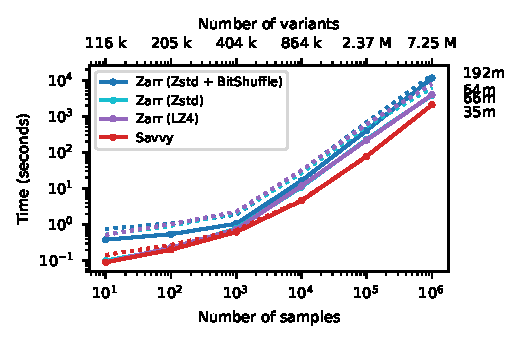
\includegraphics{figures/whole-matrix-decode}
\caption{Genotype decoding performance.
Total CPU time required to decode genotypes into memory using the zarr-python
and Savvy C++ APIs for the data in Figure~\ref{fig-data-storage}.
This corresponds to maximum rate of 1.2GiB/s for Zarr and 5.7GiB/s
for Savvy. [TODO add data for 1 million samples]
\label{fig-whole-matrix-decode}}
\end{figure}

\begin{figure}
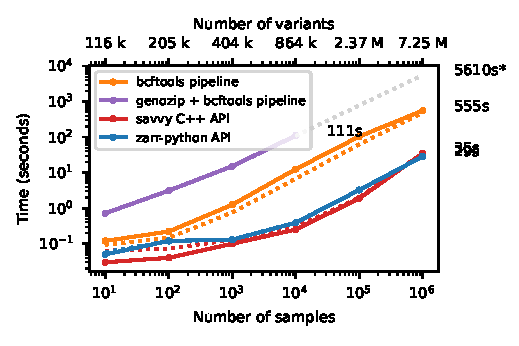
\includegraphics{figures/subset-matrix-compute-supplemental}
\caption{Compute performance on a large subset of the genotype matrix.
Total CPU time required to run the af-dist calculation for
a subset of half of the samples and 10000 variants from the middle of the matrix
for the data in Figure~\ref{fig-data-storage}.
Genozip did not run for
$n > 10^4$ samples because it does not support a file to specify
sample IDs, and the command line was therefore too long for the shell
to execute. 
\label{fig-subset-matrix-compute-supplemental}}
\end{figure}

\begin{figure}
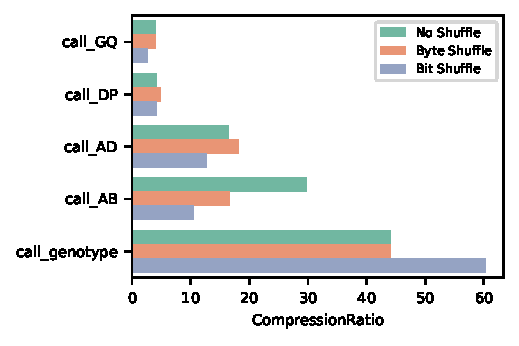
\includegraphics{figures/compression-shuffle}
\caption{Effects of shuffle setting on compression ratios on 1000 Genomes
data. TODO MORE DETAIL. 
\label{fig-compression-shuffle}}
\end{figure}

\begin{figure}
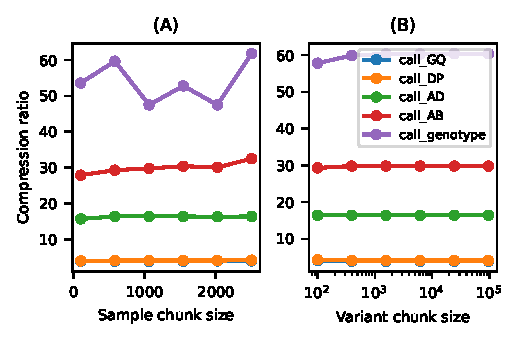
\includegraphics{figures/compression-chunksize}
\caption{Effects of chunk sizes on compression ratios on 1000 Genomes
data. TODO MORE DETAIL. 
\label{fig-compression-chunksize}}
\end{figure}

\end{document}
